%\documentclass[preprint]{aastex}  % USE THIS TO MAKE BIB, THEN FORMAT USING EMULATEAPJ
\documentclass[onecolumn]{emulateapj} \shorttitle{}
\shortauthors{Ali, et al.}

\usepackage{amsmath} \usepackage{graphicx} \usepackage[figuresright]{rotating}
\usepackage{subfig}
%\usepackage{rotating}
\usepackage{natbib}
%\usepackage{pdflscape} \usepackage{lscape}
\citestyle{aa}

\def\b{\mathbf{b}} \def\k{\mathbf{k}} \def\r{\mathbf{r}} \def\q{\mathbf{q}}
\def\b{\mathbf{b}} \def\kp{\mathbf{k}^\prime}
\def\kpp{\mathbf{k}^{\prime\prime}} \def\V{\mathbb{V}} \def\expval#1{\langle #1
\rangle} \def\At{\tilde{A}} \def\Vt{\tilde{V}} \def\Tt{\tilde{T}}
\def\tb{\langle T_b\rangle} \newcommand{\vis}{\mathbf{v}}
\newcommand{\x}{\mathbf{x}} \newcommand{\xhat}{\hat{\mathbf{x}}}
\newcommand{\A}{\mathbf{A}} \newcommand{\N}{\mathbf{N}}
\newcommand{\C}{\mathbf{C}} \newcommand{\Q}{\mathbf{Q}}
\newcommand{\rhat}{\hat{\mathbf{r}}}
\newcommand{\phat}{\hat{\mathbf{p}}}
\newcommand{\qhat}{\hat{\mathbf{q}}}
\newcommand{\hMpci}{h\ {\rm Mpc}^{-1}}
\newcommand{\Tsys}{T_{\rm sys}}
\newcommand{\Tspin}{T_{\rm s}}
\newcommand{\kmin}{k_{\rm min}}
\newcommand{\kmax}{k_{\rm max}}
\newcommand{\Tcmb}{T_\gamma}
\newcommand\abs[1]{\left|#1\right|}
\newcommand{\mKlimit}{(22.4\,\textrm{mK})$^2$ }
\newcommand{\mKsqlimit}{503 mK$^2$}
\newcommand{\revisedmklimit}{(212.2\,\textrm{mK})$^2$}
\newcommand{\pobercitep}{(Pober et al. 2015, in prep)}
\newcommand{\pobercitet}{Pober et al. (2015, in prep)}
\newcommand{\parsonscitep}{(Parsons et al. 2015, in prep)}
\newcommand{\parsonscitet}{Parsons et al. (2015, in prep)}
\newcommand{\kolopaniscitet}{Kolopanis et al. (2018, submitted)}
\newcommand{\chengcitet}{Cheng et al. (2018, submitted)}

\newcount\colveccount
\newcommand*\colvec[1]{
        \global\colveccount#1
        \begin{pmatrix}
        \colvecnext
}
\def\colvecnext#1{
        #1
        \global\advance\colveccount-1
        \ifnum\colveccount>0
                \\
                \expandafter\colvecnext
        \else
                \end{pmatrix}
        \fi
}


\begin{document}

\title{ERRATUM: "PAPER-64 Constraints on Reionization: the  $21\,\textrm{cm}$ Power Spectrum at $z=8.4$" (2015, Apj, 809, 61)}

\author{
Zaki S. Ali\altaffilmark{1}, 
Aaron R. Parsons\altaffilmark{1,2}, 
Haoxuan Zheng\altaffilmark{3},
Jonathan C. Pober\altaffilmark{4}, 
Adrian Liu\altaffilmark{1,5}, 
James E. Aguirre\altaffilmark{6},
Richard F. Bradley\altaffilmark{7,8,9},
Gianni Bernardi\altaffilmark{10,11,12}, 
Chris L. Carilli\altaffilmark{13,14},
Carina Cheng\altaffilmark{1},
David R. DeBoer\altaffilmark{2}, 
Matthew R. Dexter\altaffilmark{2},
Jasper Grobbelaar\altaffilmark{10},
Jasper Horrell\altaffilmark{10},
Daniel C. Jacobs\altaffilmark{15}, 
Pat Klima\altaffilmark{8},
David H. E. MacMahon\altaffilmark{2},
Matthys Maree\altaffilmark{10},
David F. Moore\altaffilmark{6},
Nima Razavi\altaffilmark{14},
Irina I. Stefan\altaffilmark{14},
William P. Walbrugh\altaffilmark{10},
Andre Walker\altaffilmark{10}
}
%\tableofcontents

\altaffiltext{1}{Astronomy Dept., U. California, Berkeley CA}
\altaffiltext{2}{Radio Astronomy Lab., U. California, Berkeley CA}
\altaffiltext{3}{Dept. of Physics, Massachusetts Inst. of Tech., Cambridge MA}
\altaffiltext{4}{Physics Dept.  U. Washington, Seattle WA}
\altaffiltext{5}{Berkeley Center for Cosmological Physics, Berkeley, CA} 
\altaffiltext{6}{Dept. of Physics and Astronomy, U. Penn., Philadelphia PA} 
\altaffiltext{7}{Dept. of Electrical and Computer Engineering, U. Virginia, Charlottesville VA}
\altaffiltext{8}{National Radio Astronomy Obs., Charlottesville VA}
\altaffiltext{9}{Dept. of Astronomy, U. Virginia, Charlottesville VA}
\altaffiltext{10}{Square Kilometer Array, S. Africa, Cape Town South Africa}
\altaffiltext{11}{Dept. of Physics and Electronics, Rhodes University}
\altaffiltext{12}{Harvard-Smithsonian Cen. for Astrophysics, Cambridge MA}
\altaffiltext{13}{National Radio Astronomy Obs., Socorro NM}
\altaffiltext{14}{Cavendish Lab., Cambridge UK}
\altaffiltext{15}{School of Earth and Space Exploration, Arizona State U., Tempe AZ}

% http://journals.aas.org/authors/manuscript.html says not to include an abstract, but Iv'e 
% included one here to keep our message straight. 
%\begin{abstract}
%In this erratum we update the reported upper limits on the 21cm power spectrum.
%The original results reported a $2\sigma$ upper limit on $\Delta^2(k)$ of
%\mKlimit in the range $0.15<k<0.5\hMpci$ at $z=8.4$ The revised result, found in
%\kolopaniscitet,  puts an upper limit of \revisedmklimit at$k = .3\hMpci$.
%\end{abstract}

\maketitle

In this erratum, we revise the upper limits on the 21 cm power spectrum presented
in the original manuscript.  In the original manuscript, an upper limit on 
$\Delta_{21}^2(k)$ of \mKlimit was reported at $z=8.4$ in the range $0.15<k<0.5\hMpci$.
This analysis underestimated 
the level of loss associated with the chosen power spectrum estimator and also underestimated 
the statistical error in those estimates.  The revised result, shown in Figure \ref{fig:updated_pspec}, 
which is included in
the multi-redshift limits of \kolopaniscitet, places a best upper limit of \revisedmklimit 
at $z=8.4$ and $k=0.3\hMpci$.
Below, we briefly summarize the errors in the original analysis and how they are corrected.
For an in-depth analysis of the errors, we refer the reader to \chengcitet.

The first and most impactful error relates to the method by which signal loss was estimated.
Signal loss was expected in the original analysis because the covariance matrices, $C$,
used to weight the un-normalized bandpower estimates, ${\mathbf q}_\alpha$, in
\begin{equation}
{\mathbf q}_\alpha = {\mathbf x}C_{x}^{-1}Q_\alpha C_{x}^{-1}{\mathbf x}
\end{equation} 
were empirically estimated from a finite ensemble of the data, $\mathbf x$, as $C_{x}=\langle {\mathbf x} {\mathbf x}^\dagger\rangle$.
To assess signal loss, mock cosmological signals $\mathbf e$ of known amplitudes were 
drawn with random seeds and added to the original data to form a new data vector, ${\mathbf r}\equiv{\mathbf x} + {\mathbf e}$.
New covariance matrices, $C_r=\langle{\mathbf r}\mathbf{r}^\dagger\rangle$, were used to estimate un-normalized bandpowers, 
${\mathbf q}_{\alpha,r}$. Since these bandpower estimates include contributions from both $\mathbf x$ and $\mathbf e$,
an incremental bandpower associated with $\mathbf e$ was computed as
\begin{align}
{\mathbf q}_{\alpha,e}&\equiv{\mathbf q}_{\alpha,r}-{\mathbf q}_\alpha \\
&=
{\mathbf x}C_r^{-1}Q_\alpha C_r^{-1}{\mathbf x}+
{\mathbf x}C_r^{-1}Q_\alpha C_r^{-1}{\mathbf e}+
{\mathbf e}C_r^{-1}Q_\alpha C_r^{-1}{\mathbf x}+
{\mathbf e}C_r^{-1}Q_\alpha C_r^{-1}{\mathbf e}
- {\mathbf x}C_x^{-1}Q_\alpha C_x^{-1}{\mathbf x} \\
&\approx
{\mathbf x}C_r^{-1}Q_\alpha C_r^{-1}{\mathbf e}+
{\mathbf e}C_r^{-1}Q_\alpha C_r^{-1}{\mathbf x}+
{\mathbf e}C_r^{-1}Q_\alpha C_r^{-1}{\mathbf e},
\label{eq:crossterms}
\end{align}

%ZA: I think we should add in the equation we acutally used in the signal loss, e.g. {\mathbf e}C_r^{-1}Q_\alpha C_r^{-1}{\mathbf e}
% as the last line in equation \ref{eq:crossterms} for completeness. I know it's discussed in the text, but having the equation 
% we actually used in the original signal would be good to show how far off we were.
where the last cancellation assumes that the change in weighting between $C_{x}$ and $C_r$ does not substantially change
the normalized power spectrum estimate, ${\mathbf p}=M{\mathbf q}$, for appropriate choices of the normalization matrix, $M$.
The normalized incremental power was then compared to the known injected power in $\mathbf e$ to estimate signal loss.

The key error in the previous analysis was to assume that, since $\mathbf e$ was statistically independent of $\mathbf x$, that
the $\mathbf x$-$\mathbf e$ cross-terms in Eq. (\ref{eq:crossterms}) would average to zero in an ensemble.  In fact, as shown
in \chengcitet, these terms can contain significant negative power, since $C_r$ contains information that correlate the
two vectors.  As a result, the amount of signal loss present was mis-estimated to be negligible, when in fact approximately
XXX\% of the signal had been lost. Correcting for the actual signal loss was the biggest factor revising the upper limit
on $\Delta^2_{21}$.

The second mistake made in the original analysis was to underestimate the statistical errors in the reported power spectrum
estimates.  The original analysis used a bootstrapping technique to resample power spectral measurements made as a function
of time and baseline before averaging them.  However, fringe-rate filtering introduces significant correlations in the data
along the time axis.  As is discussed in \chengcitet, bootstrapping across correlated samples results in a significant underestimate
of the variation in the data.  In this case, the error bars were underestimated by approximately a factor of 2 (XXX check this).
The revised analysis only applies bootstrap resampling across the baseline axis to avoid this problem.

The mistake in estimating the statistical errors should have become apparent when comparing results to our theoretical
thermal noise sensitivity.  Unfortunately, a third miscalculation was made in estimating the thermal noise sensitivity.
As detailed in \chengcitet, this miscalculation stemmed from numerous small mismatches between the idealized analysis
pipeline used to estimate sensitivity and the actual analysis applied to the data.  As a result, our estimated thermal
noise sensitivity was a factor of approximately 2 low, leading the the mistaken impression that our
errorbars were consistent with the level of thermal noise.

In summary, Figure \ref{fig:updated_pspec} of this erratum includes corrections to the original analysis relating to
an incorrect estimate of signal loss and a mis-estimation the the statistical error in those measurements.
These results replace the results in Figures 18 and 20 in the original manuscript.  Results that relied on
the original limits, including those presented in Figures 21, are retracted.
% XXX i don't think we can point to errors in other papers in this erratum, but should we mention Pober et al?
%ZA: I agree to the first part. I think we should probably ask Jonnie if he wants to write his own quick erratum 
% or if we should mention it here.
Our revised results are put into context with measurements at other redshifts in \kolopaniscitet.  
% XXX anything else?

\begin{figure}%
    \centering
    \subfloat[a]{{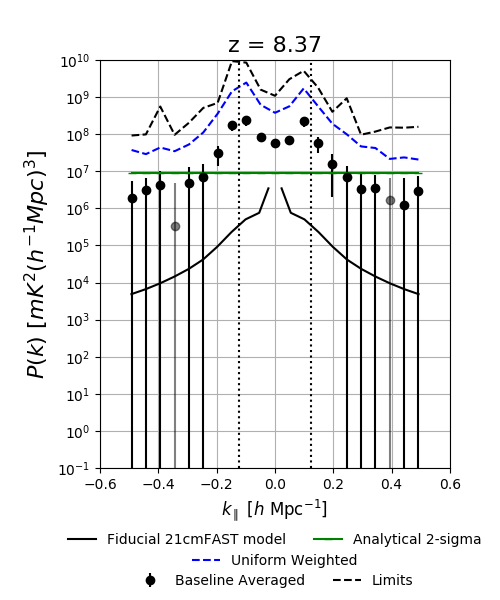
\includegraphics[width=6cm]{plots/pspec_95_pk.png} }}%
    \qquad
    \subfloat[b]{{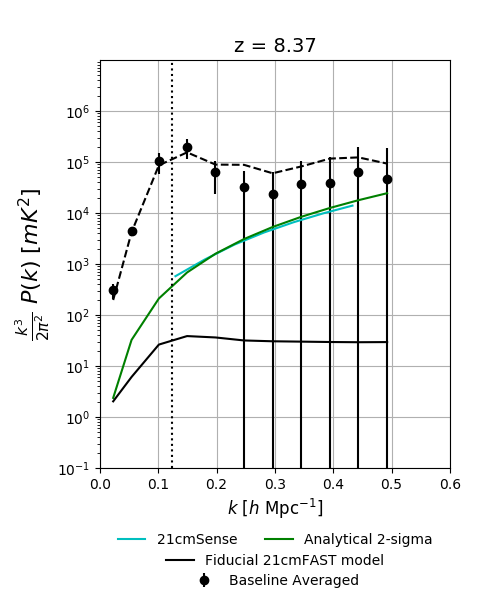
\includegraphics[width=6cm]{plots/pspec_95.png} }}%
    \caption{Measured power spectrum (black dots with 2 $\sigma$ error bars) at $z=8.37$ shown in (a) $P(k)$ and (b) $\Delta^{2}$
             Using 135 days of PAPER 64 data. The dotted vertical lines at $k=0.6$\hMpci show the bounds of the delay filter (or the horizon limit).
             Both the analytical(cyan) and 21 cmsense (green) 2$\sigma$ noise power spectrum are also shown assuming a $T_{sys}=300K (XXX)$}%
    \label{fig:updated_pspec}%
\end{figure}

%\begin{figure}\centering
%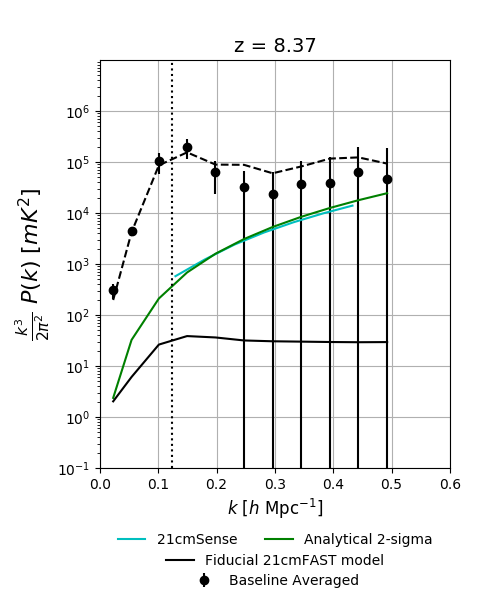
\includegraphics[width=\columnwidth, height=4in]{plots/pspec_95.png}
%%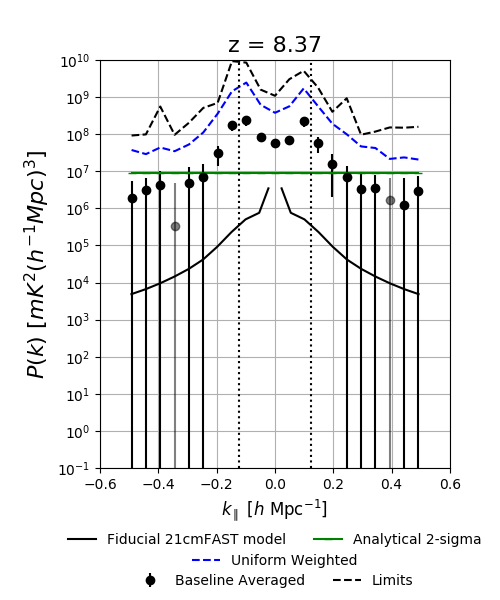
\includegraphics[width=\columnwidth]{plots/pspec_95_pk.png}
%\caption{}
%\label{fig:updataed_pspec}
%\end{figure}
\clearpage
\nocite{*}
\bibliographystyle{apj}
\bibliography{biblio}

\end{document}

